\subsection{Aim}
\begin{enumerate}[(a)]
\item To predict the angle of release of pendulum projectile by measuring range of the projectile.
\item To use the results of (a) to compare the predictions of SAA with a more accurate analysis considering the exact forces of the system. 
\end{enumerate}
\subsection{Materials Required}
Metallic bob, Thread, Iron Stand, Protractor, Metre Scale, Scissors
\subsection{Theory}
\emph{Simple harmonic motion} is a type of periodic motion where the restoring force is directly proportional to the displacement and acts in the direction opposite to that of displacement. The restoring force is given by:
\[
  \mathbf{F}=-kx
\]
where $\mathbf{F}$ is the restoring force, $k$ is a constant, and $x$ is the displacement from the equillibrium position.

A pendulum is a weight suspended from a frictionless pivot so that it can swing freely. For a pendulum to act as an SHM oscillator, the force on the weight must be proportional to the displacement of the weight from the equillibrium position. But from \textit{fig.1} it can be clearly seen that the magnitude of the restoring torque of $mg$ is given by:
\[
  |\bm{\Gamma}|=-mgl\sin\theta
\]
It is clearly seen that the restoring torque is not directly proportional to the angular displacement, which means that the pendulum is not an SHM oscillator. But for small values of $\theta$, $\sin\theta$ is approximately equal to $\theta$, and thus for this case alone does the pendulum act as an SHM. The displacement of the weight for small angles can thus be given by:
\[
  \theta=\phi\sin\omega t \numberthis \label{eqn}
\]
\cleardoublepage
where $\phi$ is the amplitude (in this case, the initial \emph{angle of release} of the pendulum), $\omega$ is the angular frequency, and $t$ is any time instant.
\\ \\
Differentiating with respect to time, we obtain:
\[
  \frac{\dd{\theta}}{\dd{t}}=\vec{\omega}=\phi\omega\cos\omega t
\]
and since the tangential velocity $v=r\omega$, in this case,
\[
  v=l\phi\omega\cos\omega t
\]
where $l$ is the length of the pendulum.
\\
Further,
\begin{align*}
  v&=l\phi\omega\sqrt{1 - \sin^2\omega t}\\
   &=l\omega\sqrt{\phi^2(1 - \sin^2\omega t)}\\
   &=l\omega\sqrt{\phi^2 - \phi^2\sin^2\omega t}\\
   &=l.\sqrt{\frac{g}{l}}\left(\sqrt{\phi^2 - \theta^2}\right) &&\text{($\because \omega=\sqrt{\frac{g}{l}}$ and 1.1)} \\
 \implies \Aboxed{v&=\sqrt{ g(\phi^2 - \theta^2) }} \numberthis \label{eqn} 
\end{align*}

We can avoid the above approximations, by considering the $\sin\theta$ term and adopting another approach through calculus to find $v$.
\\ \\ \\
From \emph{fig.1}, the tangential acceleration of the weight is given by:
  \[a_t=-g\sin\theta\]
We know that $a_t=\frac{\dd{v}}{\dd{t}}$, thus,
  \[\frac{\dd{v}}{\dd{s}}\frac{\dd{s}}{\dd{t}}=-g\sin\theta\]
Furthermore, $\frac{\dd{s}}{\dd{t}}=v$,from which we obtain
  \[v\dd{v}=-g\sin\theta\dd{s}\]
Integrating on both sides,
  \begin{align*}
    &\int_0^v v\dd{v} = -\int_\phi^\theta gl\sin\theta\dd{\theta} &&\text{($\because\dd{s}=l\dd{\theta}$)}\\
   \implies &\frac{v^2}{2} = gl[ \cos\theta ]^\theta_\phi = gl(\cos\theta - \cos\phi)\\
   \implies &\boxed{v=\sqrt{2gl( \cos\theta - \cos\phi )}} \numberthis \label{eqn} 
  \end{align*}
  (1.3) is the general expression for the velocity of the weight in a pendulum as a function of $\theta$ without any \emph{small angle approximations}.
  \cleartoleftpage
  \vspace*{6cm}
\begin{figure}[h]
  \begin{center}
    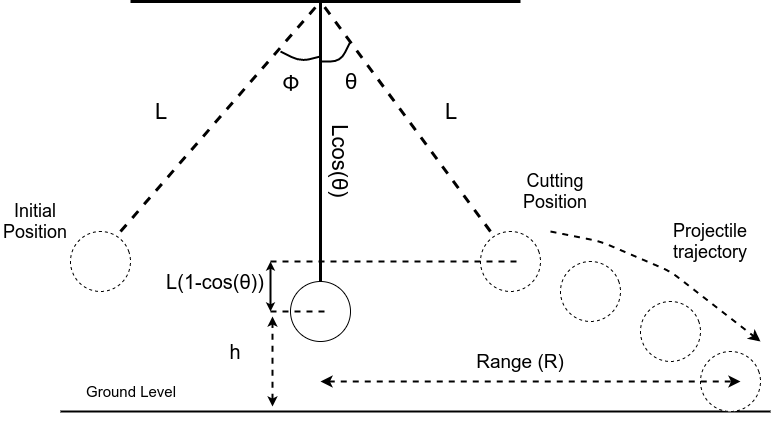
\includegraphics[width=17cm]{fig2}
    \end{center}
  \caption*{Fig.2 Experiment Diagram}
 \end{figure}
  \cleardoublepage
  Now, lets assume the string of the pendulum is cut. The velocity of the bob $v$ at the instant the string is cut is given by \emph{(1.2)} and \emph{(1.3)}. From \emph{fig.2} and projectile equations the time taken for the bob to reach maximum height is given by:
  \[t_1=\frac{v\sin\theta}{g}\]
  At the time instant $t_1$, the bob is at the maximum height in its parabolic trajectory. Thus, its total height at this moment is given by (\emph{fig.2}):
  \[d=\frac{v^2\sin^2\theta}{2g}+l(1-\cos\theta)+h\]
We know that an object at height $d$ will fall to the ground in time:
\[t_2=\sqrt{\frac{2d}{g}}\]
Thus the total time taken for the bob to reach the ground after the string is cut is:
\begin{align*}
  t&=\text{(Time taken to reach max height) + (Time taken to fall to ground from max height)}\\
     &=t_1+t_2
\end{align*}
Thus the range $r$ of the projectile (bob) is given by:
\[r=( v\cos\theta ) t\]
But, this range $r$ is relative to the position the bob was cut at. This quantity cannot be measured easily in an experimental environment. Instead, we can find the range relative to the equillibrium position of the bob, by adding $l\sin\theta$ to the range:
\begin{align*}
  R&=l\sin\theta + r \\
  &=l\sin\theta + (v\cos\theta)t \\
  \implies \Aboxed{R&=l\sin\theta + v\cos\theta\left(\frac{v\sin\theta}{g}+\sqrt{\frac{2(\frac{v^2\sin^2\theta}{2g}+l(1-\cos\theta)+h)}{g}}\:\right)} \numberthis \label{eqn}
\end{align*}
\\ \\
The first aim of this experiment is to observe readings of R, and predict the values of $\theta$ by looking at the graph of $R$ vs $\theta$ for measured values of $l$, $h$ and $\phi$. The second aim is to compare and analyse the graphs of $R$ vs $\theta$ for the two expressions for $v$ obtained above (1.2 and 1.3). 
\subsection{Procedure}
\begin{enumerate}
\item Construct a pendulum by tying a cork to one end of a string, and a bob to the other end, and then attaching the cork to an iron stand.
\item Put a metre scale on the ground, aligning its zero with the bob's equillibrium position when seen from above the bob. Ensure the metre scale is parallel to the pendulum motion of the bob.
  \cleartoleftpage
  \vspace*{10cm}
  \begin{figure}[h]
    \begin{subfigure}{9cm}
      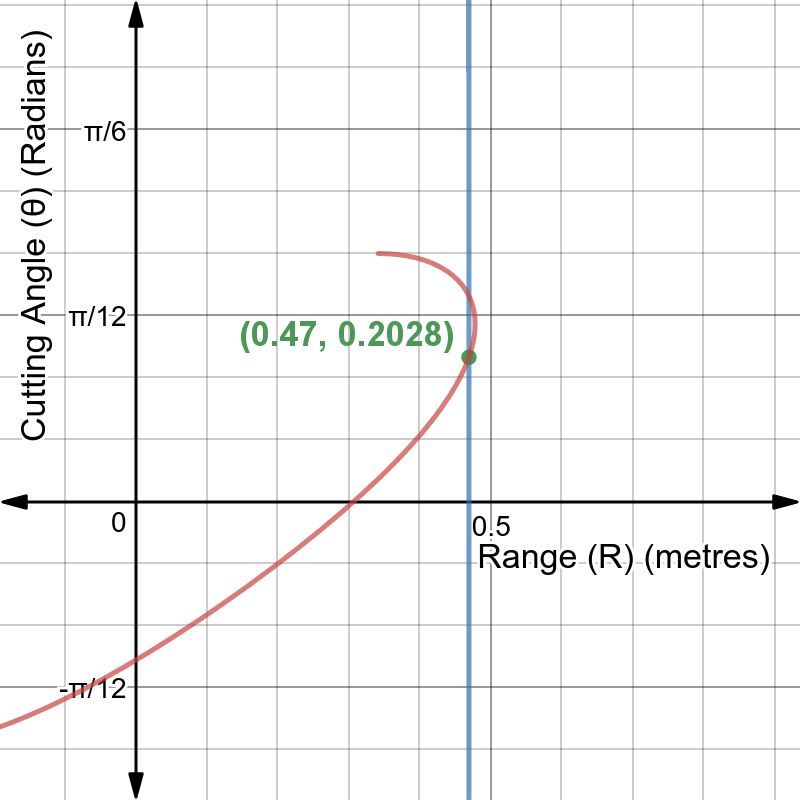
\includegraphics[width=8cm]{20deg-a}
      \caption*{(a) Approximate}
    \end{subfigure}
    \begin{subfigure}{9cm}
      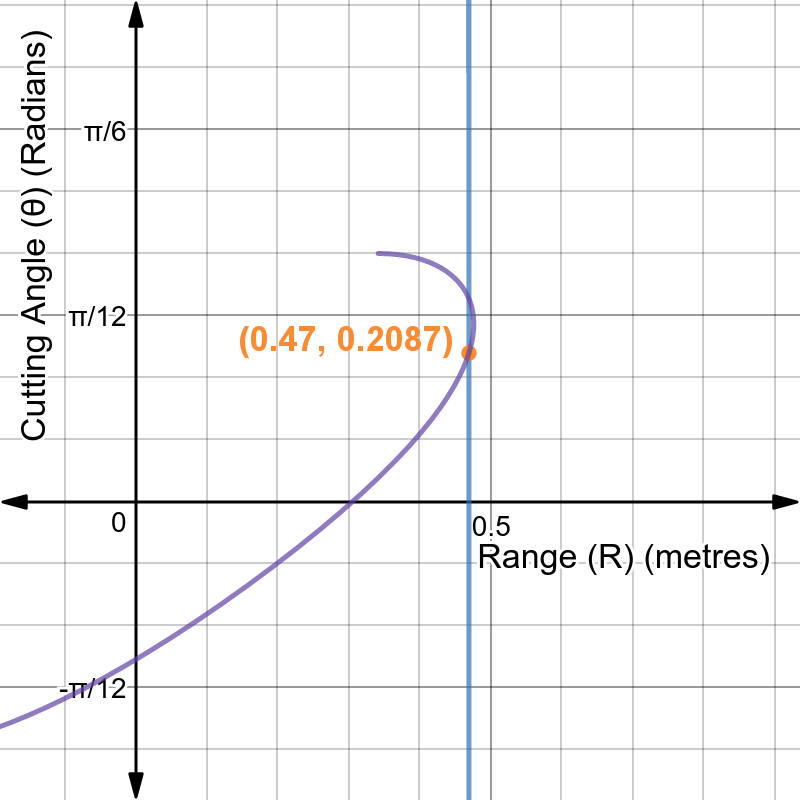
\includegraphics[width=8cm]{20deg-e}
      \caption*{(b) Real}
    \end{subfigure}
    \caption*{Graph 1: Graphs for $\phi = 20\degree$}
    \end{figure}
  \cleardoublepage
\item Ensure $l$ (length of string from the point of suspension to the centre of the bob) is 1$\mathrm{m}$.
\item Measure $h$ and note it down (length from the centre of the bob to the ground, when bob is at equllibrium)
\item Hold the bob away from its equillibrium position, and meausure the angle of release $\phi$.
\item Release the bob and cut the string with a pair of scissors at any arbitrary time in the pendulum's motion.
\item Note the range $R$ where the bob falls on the metre scale.
\item Repeat steps 3-6 for 2 more different values of the initial angle, setting up the pendulum again each time.
\end{enumerate}
\subsection{Observations}
Length of pendulum $(l)=1 \mathrm{m}$
\begin{table}[h!]
  \centering
  \begin{tabular}{|c|C{6cm}||C{4cm}|C{4cm}|@{}m{0pt}@{}}
    \hline
    \multicolumn{5}{|c|}{Observed range for different initial angles} \\
    \hline
    \textbf{No.}&\textbf{Initial Angle} $(\phi)$ (Degrees)&\textbf{Range} $(R)$ (cm)&\textbf{Height} $(h)$ (cm)&\\  [0.3cm]
    \hline
    1&$20\degree$&47&39&\\
    2&$25\degree$&54&35.5&\\
    3&$30\degree$&57&38&\\
    \hline
  \end{tabular}
\end{table}
\subsection{Graphs}
The Graphs 1, 2 and 3 correspond to the 3 observations above, each graphing the range $R$ on the x-axis, and angle of cutting $\theta$ on the y-axis.
\\ \\
Since in our proof in the theory section, we had assumed that after cutting the thread, the bob reaches maximum height first, and then falls down to the ground, we had limited our domain of observation to positive values of $\theta$, and accordingly, the given graphs should be interpreted only in the first quadrant, as the other quadrants might not relay any useful information with regard to the experiment.
\\ \\
The vertical blue line in each graph corresponds to the range found during the experiment. This line is seen to intersect for two values of $\theta$. Note that for uniformity in readings, we have arbitrarily considered the lower intersection in each case.
\\ \\
Approximate corresponds to the graph when $v$ is taken as given by (1.2), and Real corresponds to the graph when $v$ is taken as given by (1.3).
  \begin{enumerate}[\text{Graph} 1:]
  \item For $\phi=20\degree, R=0.47 \mathrm{m}$, the following values of $\theta$ are obtained:
    \begin{itemize}
    \item Approximate: $0.2028^c = 11.6196\degree$
    \item Real: $0.2087^c = 11.9575\degree$
      \cleartoleftpage
       \vspace*{1cm}
  \begin{figure}[!htb]
    \begin{subfigure}{9cm}
      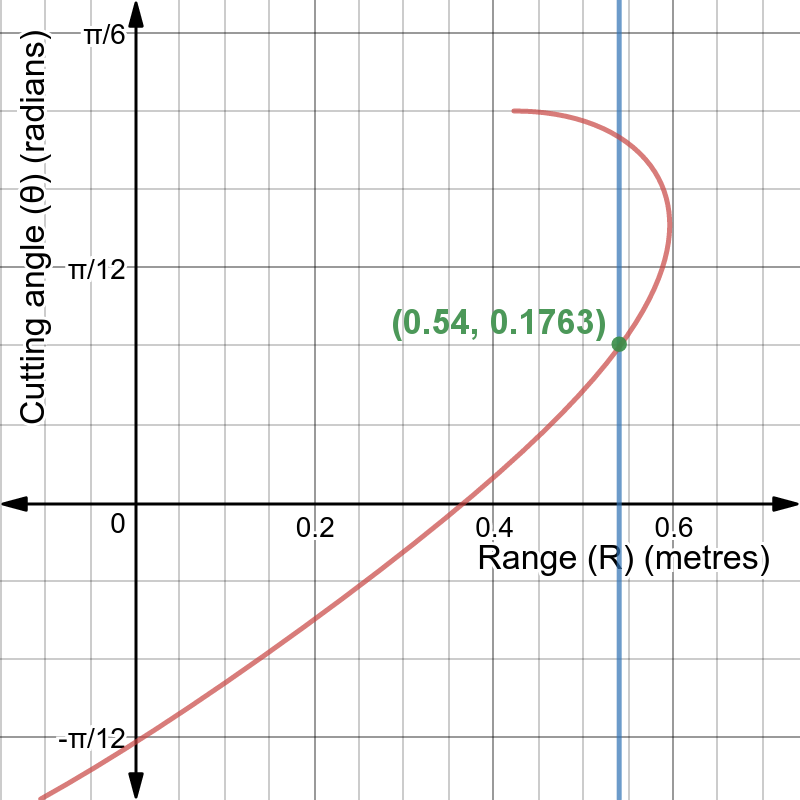
\includegraphics[width=8cm]{25deg-a}
      \caption*{(a) Approximate}
    \end{subfigure}
    \begin{subfigure}{9cm}
      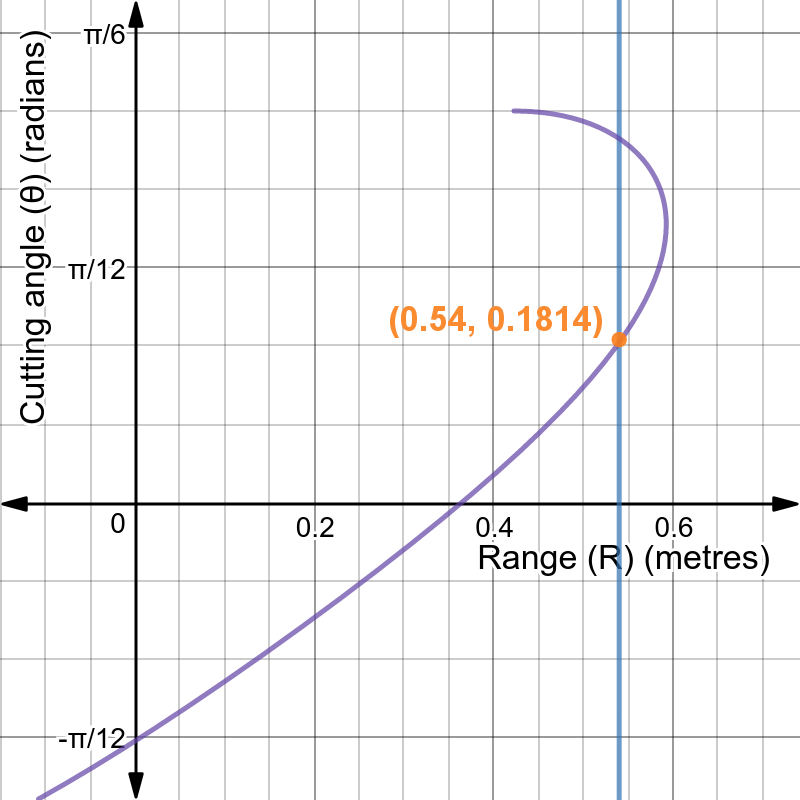
\includegraphics[width=8cm]{25deg-e}
      \caption*{(b) Real}
    \end{subfigure}
    \caption*{Graph 1: Graphs for $\phi = 25\degree$}
  \end{figure}
\vspace*{2cm}
  \begin{figure}[!htb]
    \begin{subfigure}{9cm}
      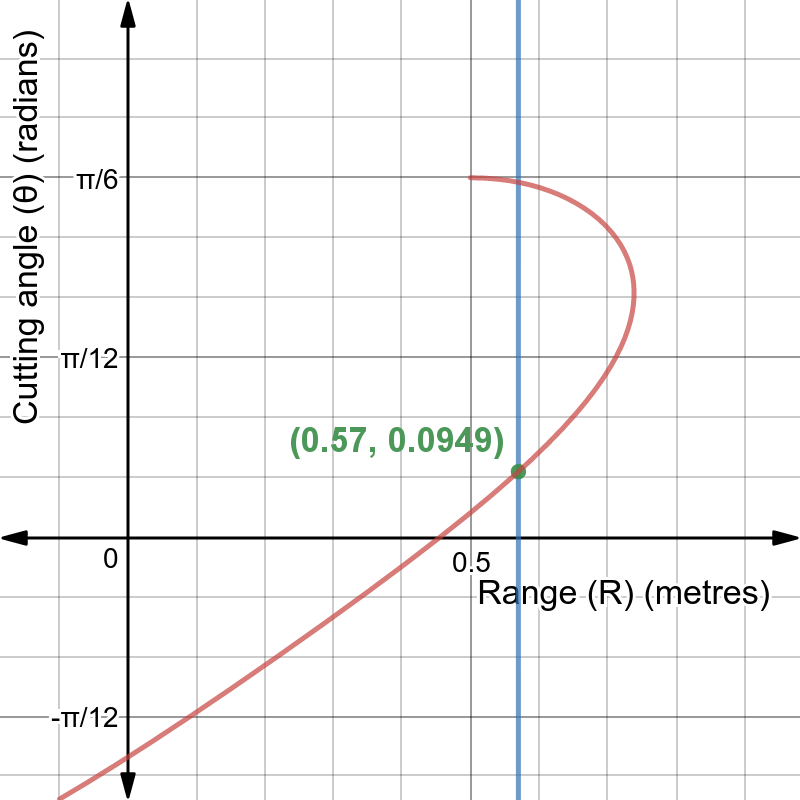
\includegraphics[width=8cm]{30deg-a}
      \caption*{(a) Approximate}
    \end{subfigure}
    \begin{subfigure}{9cm}
      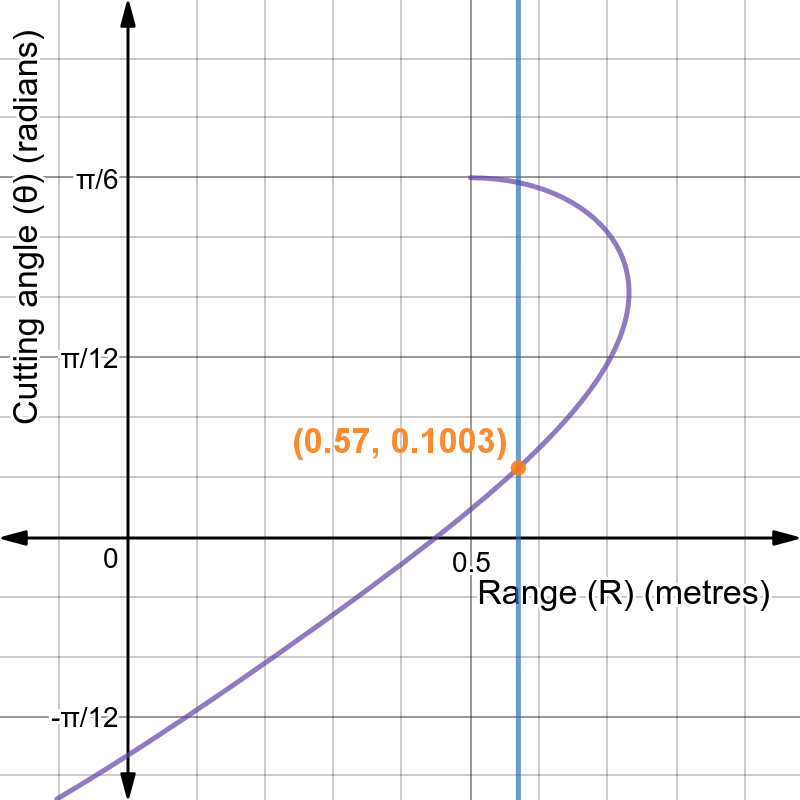
\includegraphics[width=8cm]{30deg-e}
      \caption*{(b) Real}
    \end{subfigure}
    \caption*{Graph 1: Graphs for $\phi = 30\degree$}
    \end{figure}
      \cleardoublepage
    \item Error: $0.3379$
    \item Percentage Error: $2.826 \%$ 
    \end{itemize}
  \item For $\phi=25\degree, R=0.54 \mathrm{m}$, the following values of $\theta$ are obtained:
    \begin{itemize}
    \item Approximate: $0.1763^c = 10.1011\degree$
    \item Real: $0.1814^c = 10.3934\degree$
      \item Error: $0.2923$
      \item Percentage Error: $2.812 \%$
    \end{itemize}
  \item For $\phi=30\degree, R=0.57 \mathrm{m}$, the following values of $\theta$ are obtained:
    \begin{itemize}
    \item Approximate: $0.0949^c = 5.4374\degree$
    \item Real: $0.1003^c = 5.7468\degree$
      \item Error: $0.3094$
    \item Percentage Error: $5.384 \%$
      \end{itemize}
  \end{enumerate}
  \subsection{Result}
  It is clearly seen that there is a variation between the equation of a pendulum using SAA, and the more accurate equation. It is further also seen that the error seems to increase for larger amplitudes of the pendulum.
\subsection{Precautions}
\begin{enumerate}
\item Ensure that the string has no knots, and its weight is negligible.
\item Do not cut the pendulum too late, as the amplitude might get damped, due to energy loss from friction in the air.
\item Ensure that string is cut carefully, without disturbing the oscillations in the cutting process.
\item Avoid any parallax while measuring angles/lengths.
\end{enumerate}



  

                                                                           
%%% Local Variables:
%%% mode: latex
%%% TeX-master: "../experiment"
%%% End:
